\section{Traffic Analysis}
\label{data}
For the two areas of interest, Glostrup and Herlev, TTS supplied data from detectors for a period of a couple of weeks in november 2007. 

This period is generally accepted as the beginning of the winter season and as such the traffic is expected to be high.

This is a supplement to the traffic counts, which were given by DRD. Since the detector data is anonymous with respect to vehicles types, for links in the ends of the arterial (Herlev Sygehus from north and Roskildevej from east, west and south) the data from the corresponding detectors was used in the project to scale the input sizes of the traffic counts.

The format of the data is:

\begin{table}[!ht]
\begin{center}
\begin{tabular}{c|c|c|c|c}
\textbf{Date} & \textbf{Time} & \textbf{D1} & \textbf{...} & \textbf{DN} \\ \hline
13-11-2007 & 08:42:56 & 39 & ... & 35 \\
13-11-2007 & 08:44:26 & 38 & ...  & 28 \\
\end{tabular}
\end{center}
\caption{Format of TTS supplied detector data}
\label{tab:dataformat}
\end{table}

Thus each detector, named D\textit{N}, has a column where the numbers are the detected vehicles since last detection. The detections are made once for every cycle thus there will be some variations in the time between measurements due to the adjustments to cycle time, which are made by DOGS.

It was agreed with DRD that the temporal resolution be fixed at 15 minutes. This accumulation was performed by indexing time within the data period into 15 minute bins and summing detections from the last 15 minutes.

Multiple data files - for different sets of detectors - was received for each area. Since the data period was not identical over the data files it was necessary to perform some cleanup in order to generate accumulated data in which all detectors were represented.

\begin{table}[!ht]
\begin{center}
\begin{tabular}{c|c|c|c}
\textbf{Area} & \textbf{From} & \textbf{To} & \textbf{Detectors} \\ \hline
Herlev & 13-11-2007 20:45 & 28-11-2007 09:45 & D3-D8, D13-D15, D18 \\
Glostrup & 13-11-2007 08:45 & 26-11-2007 14:15 & D1-D14 \\
\end{tabular}
\end{center}
\caption{Periods of aggregated and cleaned data sets}
\label{tab:dataperiod}
\end{table}

The cleaned data was exported to a single table of more than 30.000 rows in the format:
\begin{table}[!ht]
\begin{center}
\begin{tabular}{c|c|c|c|c|c}
\textbf{Date} & \textbf{Time} & \textbf{Area} & \textbf{Detector Name} & \textbf{From Direction} & \textbf{Vehicles} \\
\end{tabular}
\end{center}
\caption{Format of cleaned data set}
\label{tab:cleandataformat}
\end{table}

In the next section I will use the cleaned data to make some analyses and comparisons of the areas to discover facts on \textit{directional proportions} and \textit{distribution of traffic on a daily basis}.

Section \ref{traffic_count_analysis} brings additional conclusions from the traffic count data set to fill out some details, which cannot be extracted from the analysis of detector data alone.

\subsection{Detector Data Analysis}

The first four graphs (Figures \ref{fig:herlev_props_morning}-\ref{fig:glostrup_props_afternoon}) shows the overall fluctuation of traffic (mean-value) on workdays and in weekends split on mornings (7-9) and afternoons (15-17).

\begin{figure}[ht]

    \begin{minipage}[b]{0.5\linewidth}

\begin{center}
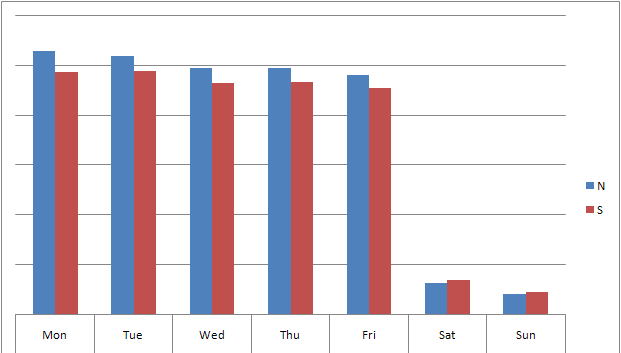
\includegraphics[scale=0.25]{herlev_direction_proportions_morning.png} 
\end{center}
\caption{Herlev - morning}
\label{fig:herlev_props_morning}

    \end{minipage}
    \hspace{0.5cm}
    \begin{minipage}[b]{0.5\linewidth}

\begin{center}
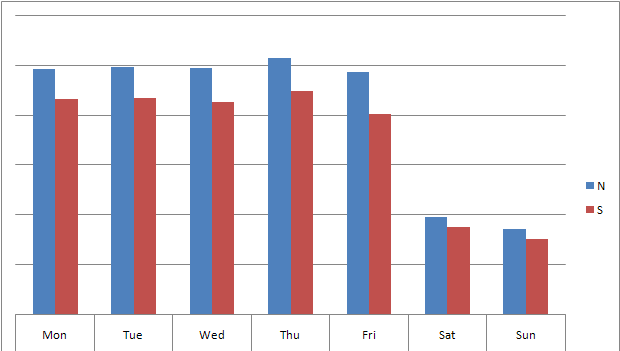
\includegraphics[scale=0.25]{herlev_direction_proportions_afternoon.png} 
\end{center}
\caption{Herlev - afternoon}
\label{fig:herlev_props_afternoon}

    \end{minipage}

\end{figure}



\begin{figure}[ht]

    \begin{minipage}[b]{0.5\linewidth}

\begin{center}
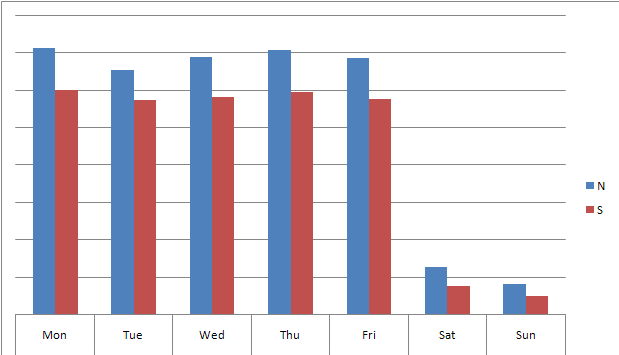
\includegraphics[scale=0.25]{glostrup_direction_proportions_morning.png} 
\end{center}
\caption{Glostrup - morning}
\label{fig:glostrup_props_morning}

    \end{minipage}
    \hspace{0.5cm}
    \begin{minipage}[b]{0.5\linewidth}
    
\begin{center}
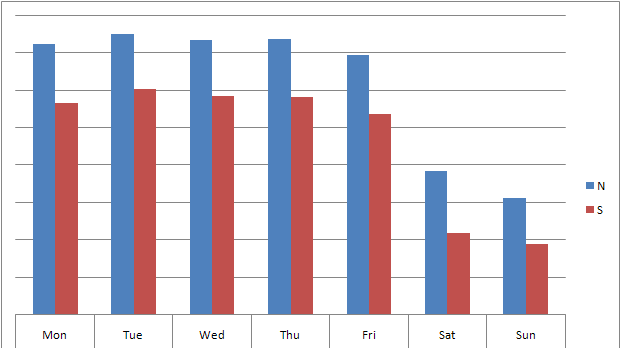
\includegraphics[scale=0.25]{glostrup_direction_proportions_afternoon.png} 
\end{center}
\caption{Glostrup - afternoon}
\label{fig:glostrup_props_afternoon}

    \end{minipage}

\end{figure}

We can see that there is an overweight of northgoing traffic. This overweight is more profound in the Glostrup area and increases in the afternoon for both areas.

From these graphs we can also see that, in the weekend, most traffic happens in the afternoon.

The next graph, see Figure \ref{fig:commuter}, shows the usual commuter- and lunch traffic patterns. The data from all mondays to fridays in the dataset have almost identical temporal distributions and thus the graph shows summarized data from workdays.

\begin{figure}[!ht]
\begin{center}
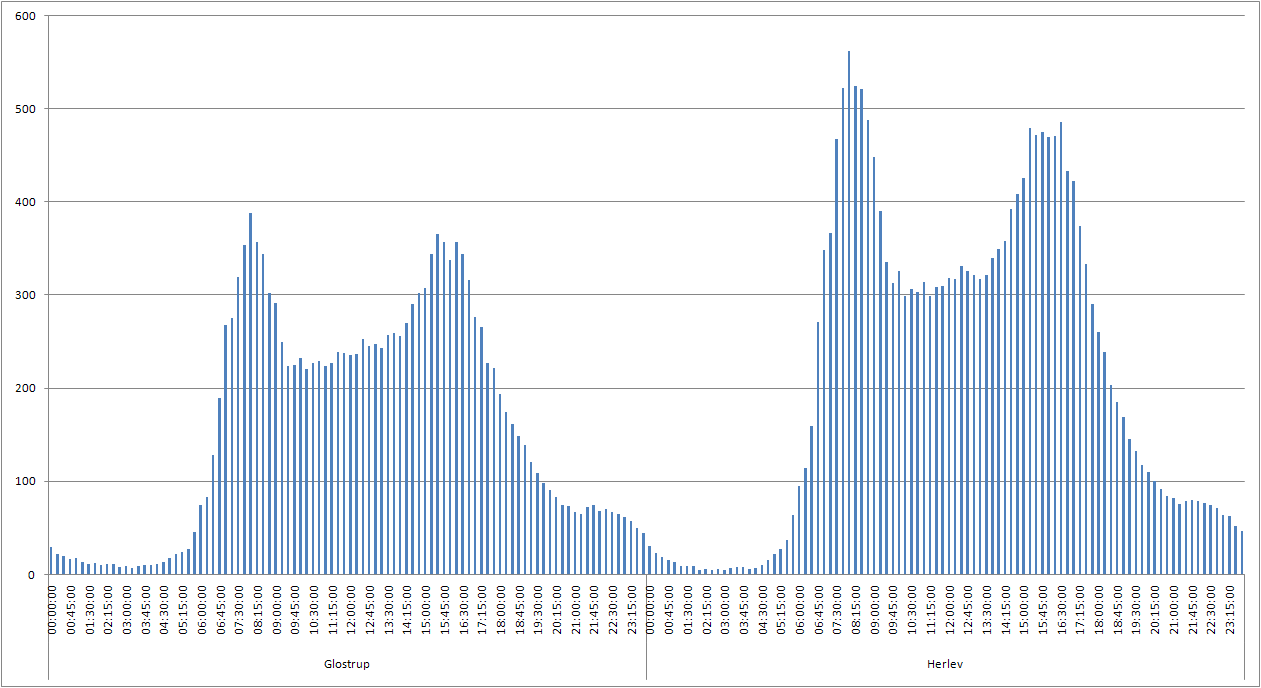
\includegraphics[scale=0.25]{distribution_workday.png} 
\end{center}
\caption{Distribution of traffic throughout workdays in Herlev and Glostrup}
\label{fig:commuter}
\end{figure}

By comparing the workday distribution to the detected traffic in the weekend, see Figure \ref{fig:weekends} - and at the same time looking and the directional proportions - it is clear that ringroad 3 is heavily used by commuters in both Herlev and Glostrup. Traffic is almost identically distributed on saturdays and sundays and the graph shows summarized data for the weekend.

\begin{figure}[!ht]
\begin{center}
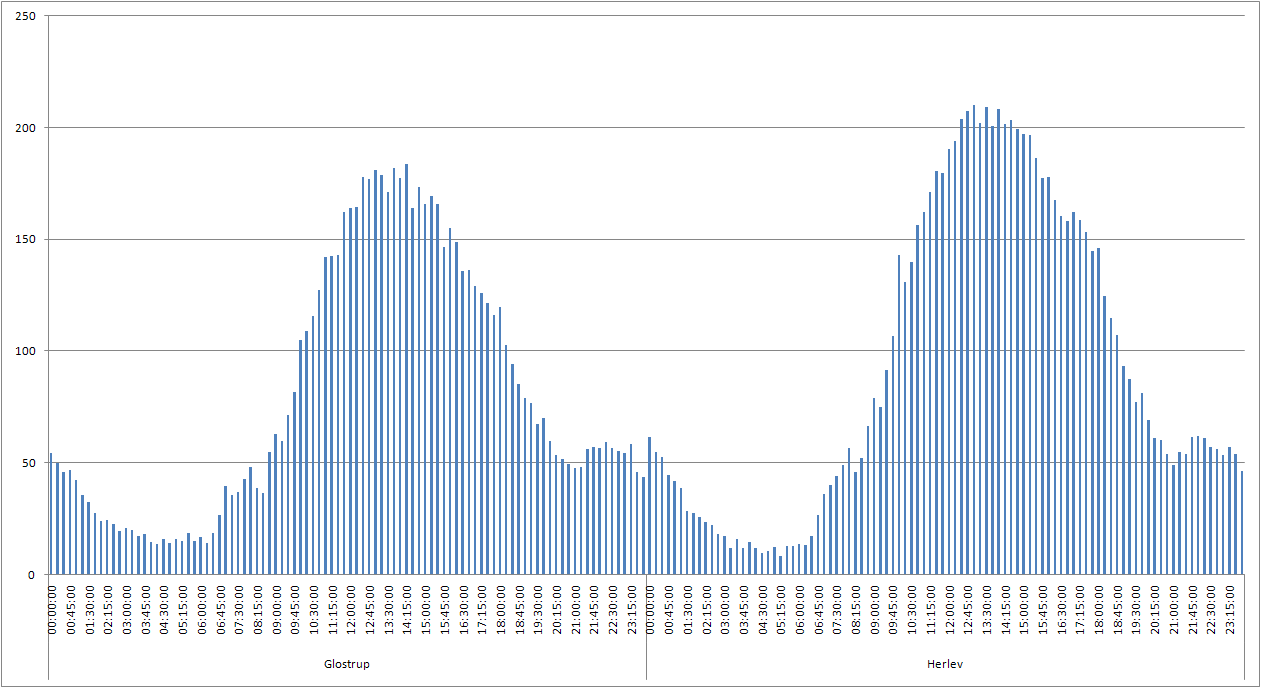
\includegraphics[scale=0.25]{distribution_weekend.png} 
\end{center}
\caption{Distribution of traffic throughout the weekend in Herlev and Glostrup}
\label{fig:weekends}
\end{figure}

The next graph (Figure \ref{fig:detector_directions}) show how detections are aligned in the north and southgoing directions in both areas. 

\begin{figure}[!ht]
\begin{center}
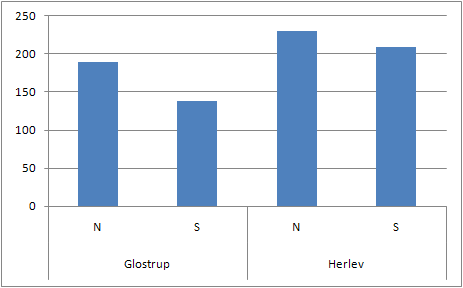
\includegraphics[scale=0.4]{detector_directions.png} 
\end{center}
\caption{Relative detections for north- and southgoing links in Herlev and Glostrup}
\label{fig:detector_directions}
\end{figure}

(For either direction and area these proportions do not vary in particular between workday and weekend.)

\subsection{Traffic Count Analysis}
\label{traffic_count_analysis}